\subsection{Controlled Contamination}
\label{sec:ctrl_contam}

We validate $\ell_z^*$ on MMLU with ground-truth contamination.
Three clean seeds yield $\ell_z^*$ values of $s_1{=}9.47$, $s_2{=}7.05$, $s_3{=}9.53$ (mean$\,{=}\,8.68\pm1.41$); $s_2$ is ${\sim}26\%$ lower than $s_1$/$s_3$, attributable to seed-specific training dynamics (Appendix~\ref{app:seed_sensitivity}).
All five conditions achieve comparable accuracy on uncontaminated items (clean $\approx$ 0.679), while contaminated models show overall accuracy gains (0.731 at 15\%, 0.764 at 50\%).

\paragraph{Finding 1: Detection signal.}
Both contamination levels produce $\ell_z^*$ shifts far exceeding clean-seed variability.
At 15\% contamination, $|\text{Cohen's}\;d|{=}3.42$; at 50\%, $|d|{=}0.99$ (ddof$\,{=}\,1$, $n{=}3$ clean seeds).
The contamination signal ($|\Delta\ell_z^*|{=}4.84$) far exceeds clean-seed variability (SD$\,{=}\,1.41$).

\paragraph{Finding 2: Free-$\theta$ non-monotonicity (model-dependent).}
Under free-$\theta$ estimation, Qwen dose-response is non-monotonic: $\Delta\ell_z^*{=}{-}4.84$ at 15\% versus ${-}1.40$ at 50\% (ratio 3.46).
The 50\% condition produces a \emph{weaker} signal because contamination inflates $\hat{\theta}_{\text{MLE}}$, absorbing part of the aberrance into a higher ability estimate ($\Delta\theta{=}0.29$ at 15\%, $0.47$ at 50\%).
This effect is model-dependent: Llama-3.1-8B shows near-monotonic free-$\theta$ dose-response (ratio 1.09) due to lower baseline misfit ($\ell_z^*{=}{-}0.14$ versus Qwen's 8.68).

\paragraph{Finding 3: Fixed $\theta$ restores monotonicity.}
We anchor at the pre-contamination baseline ($\theta_{\text{fixed}}{=}{-}0.0966$, mean of $n{=}3$ clean $\hat{\theta}$ estimates), which restores monotonic dose-response: $\Delta\ell_{z,\text{fixed}}^*{=}3.17$ (15\%) and $9.89$ (50\%), a ratio of 3.12 (Figure~\ref{fig:ctrl_contam}, right panel).

\paragraph{Finding 4: Memorization fingerprint.}
A split by seen/unseen items reveals a characteristic fingerprint: at 15\% contamination, memorized items yield $\ell_z^*{\approx}0$ (consistent with the model's inflated $\hat{\theta}$), while unseen items produce $\ell_z^*{=}3.1$, evidence of genuine aberrance on the non-memorized portion.

\paragraph{Finding 5: Memorization fraction.}
The fraction of contaminated items that the model memorizes is 0.38 (15\%) and 0.29 (50\%).
SFT generalizes beyond the memorized items, as fewer than half the injected items show rote recall.

\paragraph{Cross-family confirmation.}
Llama-3.1-8B-Instruct confirms generalizability: $|\text{Cohen's}\;d|{=}2.95$ (15\%) and $3.31$ (50\%) ($n{=}3$ clean seeds, mean$\,{=}\,{-}0.14\pm0.97$), with $|\Delta\ell_z^*|{=}2.85$ (15\%) and $3.19$ (50\%).
Unlike Qwen, Llama exhibits monotonic Cohen's $d$ dose-response ($|d|$ increases from 2.95 to 3.31), consistent with its lower baseline misfit.
Memorization fractions (0.35/0.33) and fixed-$\theta$ signal ratios (2.87) are consistent across Qwen and Llama.

Mistral-7B-Instruct ($n{=}1$ clean seed, $\ell_z^*{=}{+}5.42$) produces the strongest detection signal: $|\Delta\ell_z^*|{=}6.80$ (15\%) and $8.57$ (50\%), with monotonic dose-response.
The stronger signal likely reflects Mistral's lower baseline ability ($\text{acc}{=}0.514$, $\hat{\theta}{=}{-}1.16$), which provides greater $\theta$-shift headroom.
Because $n{=}1$, we report $\Delta\ell_z^*$ only; Cohen's $d$ requires $n \geq 2$ clean seeds.

\paragraph{Cross-family baseline divergence.}
Clean $\ell_z^*$ baselines diverge substantially: Qwen $+8.68$, Mistral $+5.42$, Llama $-0.14$.
Qwen's contaminated $\ell_z^*$ at 15\% ($+3.84$) remains positive---absolute thresholding would miss it; \irtfit{} detects contamination through the within-family shift $\Delta\ell_z^*{=}{-}4.84$.
Cohen's $d$ normalizes against clean-seed variability, yielding comparable effect sizes ($|d|{=}3.42$ vs.\ $2.95$) despite divergent baselines, confirming that \irtfit{} is a \emph{relative} detection method.

\paragraph{Baseline comparison.}
Table~\ref{tab:baseline} compares $\ell_z^*$ with alternative person-fit statistics at 15\% contamination.
$\ell_z^*$ and HT both yield large effect sizes ($|d| > 2.9$); U3 is inconsistent across families.
Item-level detection performs near random for all methods (AUROC $\leq 0.63$; Appendix~\ref{app:item_auroc}), confirming that model-level aggregation is essential.
An accuracy $z$-score yields $z{=}160$ due to near-zero cross-seed variance, but collapses in deployment (4/60 flagging rate on real data; \S\ref{sec:empirical}).

\begin{table}[t]
\centering
\caption{Model-level person-fit comparison at 15\% contamination on MMLU (Cohen's $d$, $n{=}3$ clean seeds). Item-level AUROC in Appendix~\ref{app:item_auroc}.}
\label{tab:baseline}
\footnotesize
\resizebox{\columnwidth}{!}{%
\begin{tabular}{@{}llcc@{}}
\toprule
\multicolumn{4}{@{}l}{\textit{Model-level detection (Cohen's $d$)}} \\
\midrule
Method & Info required & Qwen $d$ & Llama $d$ \\
\midrule
$\ell_z^*$ (ours) & Binary + IRT params & $\mathbf{-3.42}$ & $\mathbf{-2.95}$ \\
HT & Binary + $b$ & 3.21 & 3.53 \\
U3 & Binary + $b$ & $-$0.43 & $-$3.69 \\
Guttman errors & Binary + $b$ & --- & --- \\
\bottomrule
\end{tabular}}
\end{table}

\begin{figure*}[t]
  \centering
  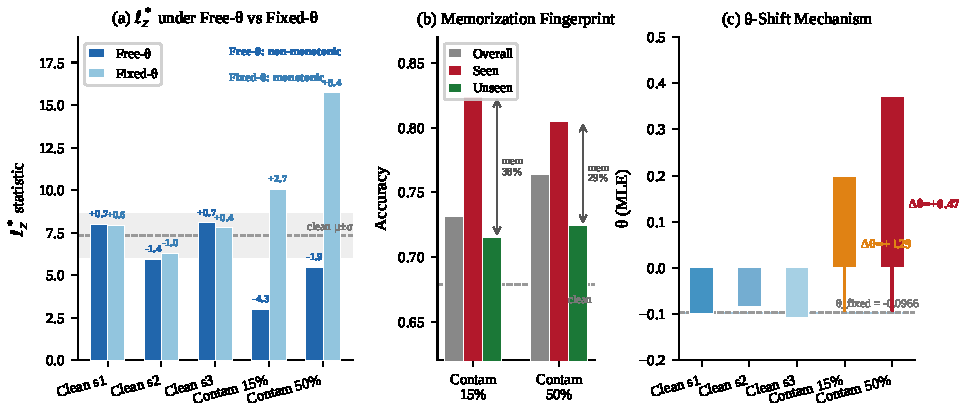
\includegraphics[width=\textwidth]{fig_3_ctrl_contam.pdf}
  \caption{Controlled contamination on MMLU. \textbf{(a)} $\ell_z^*$ under free-$\theta$ and fixed-$\theta$ estimation for five conditions (3 clean seeds, 2 contaminated). Free-$\theta$ is non-monotonic; fixed-$\theta$ restores monotonicity. \textbf{(b)} Accuracy split by seen/unseen items with memorization fractions. \textbf{(c)} $\theta$-shift mechanism: contamination inflates $\hat{\theta}_{\text{MLE}}$, absorbing aberrance signal. $\theta_{\text{fixed}}$ computed as mean of $n{=}3$ clean seed $\hat{\theta}$ estimates ($-0.0966$).}
  \label{fig:ctrl_contam}
\end{figure*}
